\section{Ice Sheet Model Intercomparison Project (ISMIP) Tests}
\subsection{Goals} %{{{
\begin{itemize}
	\item Test the ISSM skills that you have gained so far
	\item Create ISSM models by Following the given keyword instructions
	\item Run tests from the Ice Sheet Model Intercomparison Project (ISMIP - Tests A and F) (see \href{https://tc.copernicus.org/articles/2/95/2008/}{publication} for more information about these tests)
\end{itemize}

Go to \verb@trunk/examples/ISMIP/@ to do this tutorial.

%}}}
\subsection{Introduction/How To} %{{{
The \verb@runme.m@ file and \verb@*par@ files give a layout of the simulation that has to be modified.
\begin{itemize}
	\item Each code line that has to be typed in is preceded by \verb@\%->@. Type the appropriate code below this symbol.
	\item Keywords introduced by \verb@#@ should be typed in MATLAB to get more information, if necessary
	\item See the solutions below if you get stuck.
\end{itemize}
%}}}
\subsection{Test A} %{{{
In Test A, we will generate a Square ice sheet flowing over a bumpy bed:
\begin{itemize}
	\item Sinusoidal bedrock
	\item Ice frozen on the bed
	\item Periodic boundary conditions
\end{itemize}
\begin{figure}[H]
	\begin{center}
		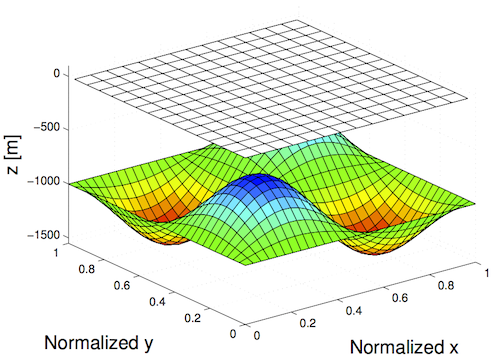
\includegraphics[scale=2.8]{/assets/img/using-issm/tutorials/ismip/SquareIceFlow.png}
	\end{center}
\end{figure}
%}}}
\subsection{Simulation File Layout and Organization}  %{{{
The simulation file \verb@runme.m@ is organized into different steps, each with the same structure:
\begin{itemize}
	\item Model loading
	\item Performing an action
	\item Model saving
\end{itemize}
The step specifier \verb@steps@ is defined at the top of the \verb@runme.m@ file.
%}}}
\subsection{Mesh} %{{{
In place of loading a preceding model we initialize one. The action here is the generation of a mesh. To do this initialize \verb@md@ as a new model \verb@(#help model)@ and generate a \verb@squaremesh@ \verb@(#help squaremesh)@ with the following parameters. Afterward, plot the mesh and save the model.
\begin{itemize}
	\item Mesh size: 80,000 meters
	\item Nodes in each direction: 20
\end{itemize}
\begin{figure}[H]
	\begin{center}
		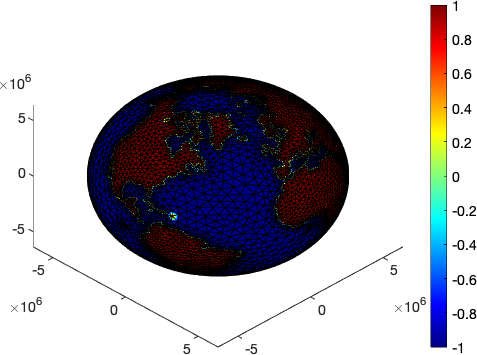
\includegraphics[scale=0.9]{/assets/img/using-issm/tutorials/ismip/Mesh.png}
	\end{center}
\end{figure}
Load the preceding step \verb@(#help loadmodel)@. Path is given by the organizer with the name of the given step. Set the mask \verb@(#help setmask)@. Note that all MISMIP nodes are grounded. Plot the given mask \verb@(md.mask)@ to locate the field. Save the model.
\begin{itemize}
	\item Mesh size: 80,000 meters
	\item Nodes in each direction: 20
	\item All grounded: default
		\end{itemize}
		\begin{figure}[H]
			\begin{center}
				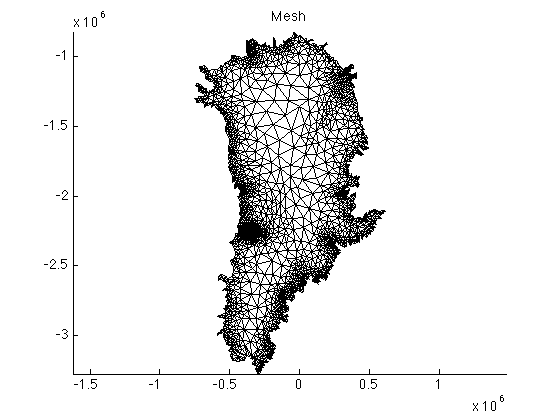
\includegraphics[scale=0.9]{/assets/img/using-issm/tutorials/ismip/Mesh2.png}
			\end{center}
		\end{figure}
		%}}}
\subsection{Parameterization} %{{{
Load the preceding step. Next, parameterize the model \verb@(#help parameterize)@. You will need to fill up the parameter file (given by the name ParamFile variable). Save the given model. It is important to note that the values are not important as we are dealing with a no-sliding flux. The values will be overridden by the basal boundary conditions. Take care of the size of the parameters.
\begin{itemize}
	\item Mesh size: 80,000 meters
	\item Nodes in each direction:20
	\item All grounded: default
	\item Ice-flow parameter: \verb@B=6.8067 x 10^7 Pa s^1/n@
	\item Glen's exponent: n=3
\end{itemize}
\begin{figure}[H]
	\begin{center}
		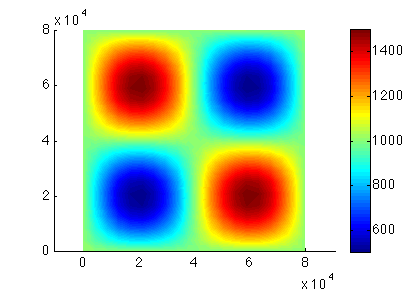
\includegraphics[scale=0.9]{/assets/img/using-issm/tutorials/ismip/Parameterize1.png}
	\end{center}
\end{figure}
%}}}
\subsection{Extrusion} %{{{
Load \verb@Parameterization@ model. The action here is to extrude the preceding mesh. Next, vertically
extrude the preceding mesh \verb@(#help extrude)@ with only 5 layers exponent 1. Plot the 3D
geometry and save the model.
\begin{itemize}
	\item Mesh size: 80,000 meters
	\item Nodes in each direction: 20
	\item All grounded: default
	\item Ice-flow parameter: \verb@B=6.8067 x 10^7 Pa s^1/n@
	\item Glen's exponent: n=3
	\item 5 layer extrusion
\end{itemize}
\begin{figure}[H]
	\begin{center}
		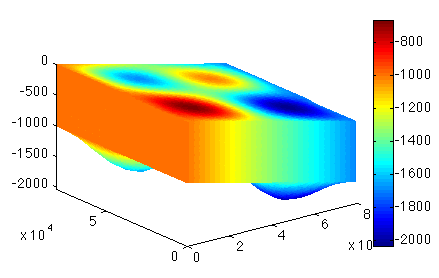
\includegraphics[scale=0.9]{/assets/img/using-issm/tutorials/ismip/Extrusion1.png}
	\end{center}
\end{figure}
%}}}
\subsection{Flow Equation} %{{{
Load the \verb@Extrusion@ model and set the approximation for the flow computation \verb@(#help setflowequation)@. We will be using the Higher Order Model (HO). Save the model.
\begin{itemize}
	\item Mesh size: 80,000 meters
	\item Nodes in each direction: 20
	\item All grounded: default
	\item Ice-flow parameter: \verb@B=6.8067 x 10^7 Pa s^1/n@
	\item Glen's exponent: n=3
	\item 5 layers extrusion
	\item Flow model: HO
\end{itemize}
%}}}
\subsection{Boundary Conditions} %{{{
Load the \verb@SetFlow@ model. Dirichlet boundary condition are known as SPC's, where ice is frozen to the base with no velocity. SPC's are initialized at NaN one value per vertex. Extract the nodenumbers at the base \verb@(#md.mesh.vertexonbase)@ and set the sliding to zero on the bed (Vx and Vy). Periodic boundaries have to be fixed on the sides. Create tabs with the side of the domain for x, and create maxX \verb@(#help find)@. This command give subsets of matrices based on boolean operations. Now create minX. For y, max X and min X should be excluded. Now create min Y. Set the node that should be paired together \verb@(#md.stressbalance.vertex_pairing)@. If we are dealing with IsmipF the solution is in masstransport. Save the given model. \verb@(#md.masstransport.vertex_pairing=md.stressbalance.vertex_pairing)@.
\begin{itemize}
	\item Mesh size: 80,000 meters
	\item Nodes in each direction: 20
	\item All grounded: default
	\item Ice-flow parameter: \verb@B=6.8067 x 10^6 Pa s^1/n@
	\item Glen's exponent: n=3
	\item 5 layer extrusion
	\item Flow model: HO
\end{itemize}
%}}}
\subsection{Solve Model} %{{{
Load the \verb@BoundaryConditions@ model. Set the cluster \verb@(#md.cluster)@ with generic parameters \verb@(#help generic)@. Set only the name and number of processes. Set which control message you want to see \verb@(#help verbose.)@ Solve \verb@(#help solve)@. We are solving a StressBalance. Save the model, and plot the surface velocities.
\begin{itemize}
	\item Mesh size: 80,000 meters
	\item Nodes in each direction: 20
	\item All grounded: default
	\item Ice-flow parameter: \verb@B=6.8067 x 10^7 Pa s^1/n@
	\item Glen's exponent: n=3
	\item 5 layers extrusion
	\item Flow model: HO
\end{itemize}
\begin{figure}[H]
	\begin{center}
		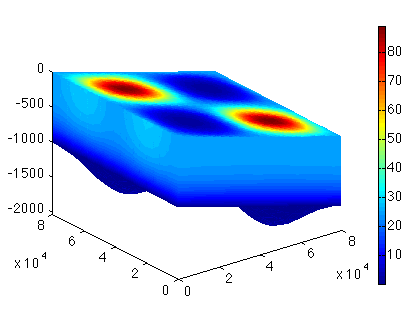
\includegraphics[scale=0.9]{/assets/img/using-issm/tutorials/ismip/BoundaryCondition.png}
	\end{center}
\end{figure}
%}}}
\subsection{Test F} %{{{
Square ice sheet flowing over a bump.
\begin{itemize}
	\item Gaussian bumped bedrock
	\item Ice frozen or sliding on the bed
	\item Periodic boundary conditions
	\item Transient model until steady-state
\end{itemize}
\begin{figure}[H]
	\begin{center}
		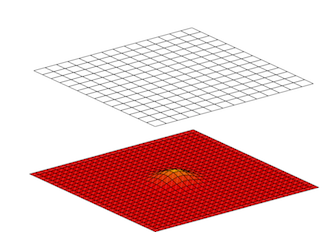
\includegraphics[scale=2.7]{/assets/img/using-issm/tutorials/ismip/RedSquareFlow.png}
	\end{center}
\end{figure}
\subsubsection{Model Setup}
\begin{itemize}
	\item Mesh size: 100,000 meters
	\item Nodes in each direction: 30
	\item All grounded: default
	\item Ice-flow parameter: \verb@B=1.4734 x 10^14 Pa s^1/n@ (or, \verb@B=A^(-1/n)@ where \verb@n=1@ and \verb@A=2.140373 x 10^-7 Pa^-1 yr^-1@)
	\item Glen's exponent: n=1
	\item 5 layers extrusion
	\item Flow model: HO
\end{itemize}
%}}}
\subsection{Actual Work and Results} %{{{
Load the preceding model under the path given by the organizer with the name of the given step. Set the cluster with generic parameters. Set only the name and number of the process. Set which control message you want to see. Set the transient model to ignore the thermal model \verb@(#md.transient)@. Define the timestepping scheme. Everything here should be provided in years \verb@(#md.timestepping)@. Give the length of the \verb@time step@ (4 years). Give the \verb@final_time (20*4 years time_steps)@. Now solve, we are solving for TransientSolution. Lastly plot the surface velocities. Here is the upper surface velocity:

Side view:
\begin{figure}[H]
	\begin{center}
		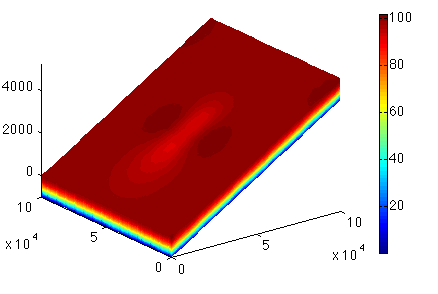
\includegraphics[scale=0.8]{/assets/img/using-issm/tutorials/ismip/UpperSurface2.png}
	\end{center}
\end{figure}
Top view:
\begin{figure}[H]
	\begin{center}
		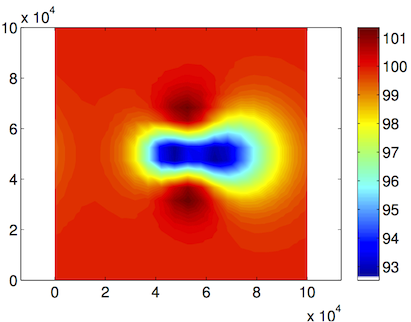
\includegraphics[scale=2.7]{/assets/img/using-issm/tutorials/ismip/UpperSurfaceVelocity.png}
	\end{center}
\end{figure}
%}}}
\subsection{Solution for runme.m (MATLAB)}%{{{
\begin{verbatim}%which steps to perform; steps are from 1 to 8
%step 7 is specific to ISMIPA
%step 8 is specific to ISMIPF

steps=[1:7]; %ISMIPA
%steps=[1:6,8]; %ISMIPB

% parameter file to be used, choose between IsmipA.par or IsmipF.par
ParamFile='IsmipA.par'
%ParamFile='IsmipF.par'

%Run Steps

%Mesh Generation #1
if any(steps==1)
	%initialize md as a new model #help model
	%->
	md=model();
	% generate a squaremesh #help squaremesh
	% Side is 80 km long with 20 points
	%->
	if(ParamFile=='IsmipA.par'),
		md=squaremesh(md,80000,80000,20,20);
	elseif(ParamFile=='IsmipF.par'),
		md=squaremesh(md,100000,100000,30,30);
	end
	% plot the given mesh #plotdoc
	%->
	plotmodel(md,'data','mesh')
	% save the given model
	%->
	save ./Models/ISMIP.Mesh_generation md;
end

%Masks #2
if any(steps==2)
	% load the preceding step #help loadmodel
	% path is given by the organizer with the name of the given step
	%->
	md = loadmodel('./Models/ISMIP.Mesh_generation');
	% set the mask #help setmask
	% all MISMIP nodes are grounded
	%->
	md=setmask(md,'','');
	% plot the given mask #md.mask to locate the field
	%->
	plotmodel(md,'data',md.mask.ocean_levelset);
	% save the given model
	%->
	save ./Models/ISMIP.SetMask md;
end

%Parameterization #3
if any(steps==3)
	% load the preceding step #help loadmodel
	% path is given by the organizer with the name of the given step
	%->
	md = loadmodel('./Models/ISMIP.SetMask');
	% parametrize the model # help parameterize
	% you will need to fill up the parameter file defined by the
	% ParamFile variable
	%->
	md=parameterize(md,ParamFile);
	% save the given model
	%->
	save ./Models/ISMIP.Parameterization md;
end

%Extrusion #4
if any(steps==4)
	
	% load the preceding step #help loadmodel
	% path is given by the organizer with the name of the given step
	%->
	md = loadmodel('./Models/ISMIP.Parameterization');
	% vertically extrude the preceding mesh #help extrude
	% only 5 layers exponent 1
	%->
	md=extrude(md,5,1);
	% plot the 3D geometry #plotdoc
	%->
	plotmodel(md,'data',md.geometry.base)
	% save the given model
	%->
	save ./Models/ISMIP.Extrusion md;
end

%Set the flow computing method #5
if any(steps==5)

	% load the preceding step #help loadmodel
	% path is given by the organizer with the name of the given step
	%->
	md = loadmodel('./Models/ISMIP.Extrusion');
	% set the approximation for the flow computation #help setflowequation
	% We will be using the Higher Order Model (HO)
	%->
	md=setflowequation(md,'HO','all');
	% save the given model
	%->
	save ./Models/ISMIP.SetFlow md;
end

%Set Boundary Conditions #6
if any(steps==6)

	% load the preceding step #help loadmodel
	% path is given by the organizer with the name of the given step
	%->
	md = loadmodel('./Models/ISMIP.SetFlow');
	% dirichlet boundary condition are known as SPCs
	% ice frozen to the base, no velocity	#md.stressbalance
	% SPCs are initialized at NaN one value per vertex
	%->
	md.stressbalance.spcvx=NaN*ones(md.mesh.numberofvertices,1);
	%->
	md.stressbalance.spcvy=NaN*ones(md.mesh.numberofvertices,1);
	%->
	md.stressbalance.spcvz=NaN*ones(md.mesh.numberofvertices,1);
	% extract the nodenumbers at the base #md.mesh.vertexonbase
	%->
	basalnodes=find(md.mesh.vertexonbase);
	% set the sliding to zero on the bed
	%->
	md.stressbalance.spcvx(basalnodes)=0.0;
	%->
	md.stressbalance.spcvy(basalnodes)=0.0;
	% periodic boundaries have to be fixed on the sides
	% Find the indices of the sides of the domain, for x and then for y
	% for x
	% create maxX, list of indices where x is equal to max of x (use >> help find)
	%->
	maxX=find(md.mesh.x==max(md.mesh.x));
	% create minX, list of indices where x is equal to min of x
	%->
	minX=find(md.mesh.x==min(md.mesh.x));
	% for y
	% create maxY, list of indices where y is equal to max of y
	%  but not where x is equal to max or min of x
	% (i.e, indices in maxX and minX should be excluded from maxY and minY)
	%->
	maxY=find(md.mesh.y==max(md.mesh.y) & md.mesh.x~=max(md.mesh.x) & md.mesh.x~=min(md.mesh.x));
	% create minY, list of indices where y is equal to max of y
	% but not where x is equal to max or min of x
	%->
	minY=find(md.mesh.y==min(md.mesh.y) & md.mesh.x~=max(md.mesh.x) & md.mesh.x~=min(md.mesh.x));
	% set the node that should be paired together, minX with maxX and minY with maxY
	% #md.stressbalance.vertex_pairing
	%->
	md.stressbalance.vertex_pairing=[minX,maxX;minY,maxY];
	if (ParamFile=='IsmipF.par')
		% if we are dealing with IsmipF the solution is in
		% masstransport
		md.masstransport.vertex_pairing=md.stressbalance.vertex_pairing;
	end
	% save the given model
	%->
	save ./Models/ISMIP.BoundaryCondition md;
end

%Solving #7
if any(steps==7)
	% load the preceding step #help loadmodel
	% path is given by the organizer with the name of the given step
	%->
	md = loadmodel('./Models/ISMIP.BoundaryCondition');
	% Set cluster #md.cluster
	% generic parameters #help generic
	% set only the name and number of process
	%->
	md.cluster=generic('name',oshostname(),'np',2);
	% Set which control message you want to see #help verbose
	%->
	md.verbose=verbose('convergence',true);
	% Solve #help solve
	% we are solving a StressBalanc
	%->
	md=solve(md,'Stressbalance');
	% save the given model
	%->
	save ./Models/ISMIP.StressBalance md;
	% plot the surface velocities #plotdoc
	%->
	plotmodel(md,'data',md.results.StressbalanceSolution.Vel)
end

%Solving #8
if any(steps==8)
	% load the preceding step #help loadmodel
	% path is given by the organizer with the name of the given step
	%->
	md = loadmodel('./Models/ISMIP.BoundaryCondition');
	% Set cluster #md.cluster
	% generic parameters #help generic
	% set only the name and number of process
	%->
	md.cluster=generic('name',oshostname(),'np',2);
	% Set which control message you want to see #help verbose
	%->
	md.verbose=verbose('convergence',true);
	% set the transient model to ignore the thermal model
	% #md.transient
	%->
	md.transient.isthermal=0;
	% define the timestepping scheme
	% everything here should be provided in years #md.timestepping
	% give the length of the time_step (4 years)
	%->
	md.timestepping.time_step=4;
	% give final_time (20*4 years time_steps)
	%->
	md.timestepping.final_time=4*20;
	% Solve #help solve
	% we are solving a TransientSolution
	%->
	md=solve(md,'Transient');
	% save the given model
	%->
	save ./Models/ISMIP.Transient md;
	% plot the surface velocities #plotdoc
	%->
	plotmodel(md,'data',md.results.TransientSolution(20).Vel)
end\end{verbatim}
%}}}
\subsection{Solution for runme.m (Python)}%{{{
\begin{verbatim}import numpy as np
from model import *
from squaremesh import squaremesh
from plotmodel import plotmodel
from export_netCDF import export_netCDF
from loadmodel import loadmodel
from setmask import setmask
from parameterize import parameterize
from setflowequation import setflowequation
from socket import gethostname
from solve import solve

#which steps to perform; steps are from 1 to 8
#step 7 is specific to ISMIPA
#step 8 is specific to ISMIPF

steps = [1, 2, 3, 4, 5, 6, 8]

# parameter file to be used, choose between IsmipA_cor.py or IsmipF_cor.py
ParamFile = 'IsmipF_cor.py'

#Run Steps

#Mesh Generation #1
if 1 in steps:
    print("Now generating the mesh")
    #initialize md as a new model help(model)
    #->
    md = model()
    # generate a squaremesh help(squaremesh)
    # Side is 80 km long with 20 points
    #->
    if ParamFile == 'IsmipA_cor.py':
        md = squaremesh(md, 80000, 80000, 20, 20)
    elif ParamFile == 'IsmipF_cor.py':
        md = squaremesh(md, 100000, 100000, 30, 30)

    # plot the given mesh plotdoc()
    #->
    plotmodel(md, 'data', 'mesh', 'figure', 1)
    # save the given model
    #->
    export_netCDF(md, "./Models/ISMIP-Mesh_generation.nc")

#Masks #2
if 2 in steps:
    print("Setting the masks")
    # load the preceding step help(loadmodel)
    # path is given by the organizer with the name of the given step
    #->
    md = loadmodel("./Models/ISMIP-Mesh_generation.nc")
    # set the mask help(setmask)
    # all MISMIP nodes are grounded
    #->
    md = setmask(md, '', '')
    # plot the given mask #md.mask to locate the field
    #->
    plotmodel(md, 'data', md.mask.ocean_levelset, 'figure', 2)
    # save the given model
    #->
    export_netCDF(md, "./Models/ISMIP-SetMask.nc")

#Parameterization #3
if 3 in steps:
    print("Parameterizing")
    # load the preceding step #help loadmodel
    # path is given by the organizer with the name of the given step
    #->
    md = loadmodel("./Models/ISMIP-SetMask.nc")
    # parametrize the model # help parameterize
    # you will need to fill up the parameter file (given by the
    # ParamFile variable)
    #->
    md = parameterize(md, ParamFile)
    # save the given model
    #->
    export_netCDF(md, "./Models/ISMIP-Parameterization.nc")

#Extrusion #4
if 4 in steps:
    print("Extruding")
    # load the preceding step #help loadmodel
    # path is given by the organizer with the name of the given step
    #->
    md = loadmodel("./Models/ISMIP-Parameterization.nc")
    # vertically extrude the preceding mesh #help extrude
    # only 5 layers exponent 1
    #->
    md = md.extrude(5, 1)
    # plot the 3D geometry #plotdoc
    #->
    plotmodel(md, 'data', md.geometry.base, 'figure', 3)
    # save the given model
    #->
    export_netCDF(md, "./Models/ISMIP-Extrusion.nc")

#Set the flow computing method #5
if 5 in steps:
    print("setting flow approximation")
    # load the preceding step #help loadmodel
    # path is given by the organizer with the name of the given step
    #->
    md = loadmodel("./Models/ISMIP-Extrusion.nc")
    # set the approximation for the flow computation #help setflowequation
    # We will be using the Higher Order Model (HO)
    #->
    md = setflowequation(md, 'HO', 'all')
    # save the given model
    #->
    export_netCDF(md, "./Models/ISMIP-SetFlow.nc")

#Set Boundary Conditions #6
if 6 in steps:
    print("setting boundary conditions")
    # load the preceding step #help loadmodel
    # path is given by the organizer with the name of the given step
    #->
    md = loadmodel("./Models/ISMIP-SetFlow.nc")
    # dirichlet boundary condition are known as SPCs
    # ice frozen to the base, no velocity   #md.stressbalance
    # SPCs are initialized at NaN one value per vertex
    #->
    md.stressbalance.spcvx = np.nan * np.ones((md.mesh.numberofvertices))
    #->
    md.stressbalance.spcvy = np.nan * np.ones((md.mesh.numberofvertices))
    #->
    md.stressbalance.spcvz = np.nan * np.ones((md.mesh.numberofvertices))
    # extract the nodenumbers at the base #md.mesh.vertexonbase
    #->
    basalnodes = np.nonzero(md.mesh.vertexonbase)
    # set the sliding to zero on the bed (Vx and Vy)
    #->
    md.stressbalance.spcvx[basalnodes] = 0.0
    #->
    md.stressbalance.spcvy[basalnodes] = 0.0
    # periodic boundaries have to be fixed on the sides
    # Find the indices of the sides of the domain, for x and then for y
    # for x
    # create maxX, list of indices where x is equal to max of x (use >> help find)
    #->
    maxX = np.squeeze(np.nonzero(md.mesh.x == np.nanmax(md.mesh.x)))
    # create minX, list of indices where x is equal to min of x
    #->
    minX = np.squeeze(np.nonzero(md.mesh.x == np.nanmin(md.mesh.x)))
    # for y
    # create maxY, list of indices where y is equal to max of y
    # but not where x is equal to max or min of x
    # (i.e, indices in maxX and minX should be excluded from maxY and minY)
    #->
    maxY = np.squeeze(np.nonzero(np.logical_and.reduce((md.mesh.y == np.nanmax(md.mesh.y), md.mesh.x != np.nanmin(md.mesh.x), md.mesh.x != np.nanmax(md.mesh.x)))))
    # create minY, list of indices where y is equal to max of y
    # but not where x is equal to max or min of x
    #->
    minY = np.squeeze(np.nonzero(np.logical_and.reduce((md.mesh.y == np.nanmin(md.mesh.y), md.mesh.x != np.nanmin(md.mesh.x), md.mesh.x != np.nanmax(md.mesh.x)))))
    # set the node that should be paired together, minX with maxX and minY with maxY
    # #md.stressbalance.vertex_pairing
    #->
    md.stressbalance.vertex_pairing = np.hstack((np.vstack((minX + 1, maxX + 1)), np.vstack((minY + 1, maxY + 1)))).T
    if ParamFile == 'IsmipF_cor.py':
        # if we are dealing with IsmipF the solution is in masstransport
        md.masstransport.vertex_pairing = md.stressbalance.vertex_pairing

    # save the given model
    #->
    export_netCDF(md, "./Models/ISMIP-BoundaryCondition.nc")

#Solving #7
if 7 in steps:
    print("running the solver for the A case")
    # load the preceding step #help loadmodel
    # path is given by the organizer with the name of the given step
    #->
    md = loadmodel("./Models/ISMIP-BoundaryCondition.nc")
    # Set cluster #md.cluster
    # generic parameters #help generic
    # set only the name and number of process
    #->
    md.cluster = generic('name', gethostname(), 'np', 2)
    # Set which control message you want to see #help verbose
    #->
    md.verbose = verbose('convergence', True)
    # Solve #help solve
    # we are solving a StressBalance
    #->
    md = solve(md, 'Stressbalance')
    # save the given model
    #->
    export_netCDF(md, "./Models/ISMIP-StressBalance.nc")
    # plot the surface velocities #plotdoc
    #->
    plotmodel(md, 'data', md.results.StressbalanceSolution.Vel, 'figure', 4)

#Solving #8
if 8 in steps:
    print("running the solver for the F case")
    # load the preceding step #help loadmodel
    # path is given by the organizer with the name of the given step
    #->
    md = loadmodel("./Models/ISMIP-BoundaryCondition.nc")
    # Set cluster #md.cluster
    # generic parameters #help generic
    # set only the name and number of process
    #->
    md.cluster = generic('name', gethostname(), 'np', 2)
    # Set which control message you want to see #help verbose
    #->
    md.verbose = verbose('convergence', True)
    # set the transient model to ignore the thermal model
    # #md.transient
    #->
    md.transient.isthermal = 0
    # define the timestepping scheme
    # everything here should be provided in years #md.timestepping
    # give the length of the time_step (4 years)
    #->
    md.timestepping.time_step = 1
    # give final_time (20*4 years time_steps)
    #->
    md.timestepping.final_time = 1 * 20
    # Solve #help solve
    # we are solving a TransientSolution
    #->
    md = solve(md, 'Transient')
    # save the given model
    #->
    export_netCDF(md, "./Models/ISMIP-Transient.nc")
    # plot the surface velocities #plotdoc
    #->
    plotmodel(md, 'data', md.results.TransientSolution[19].Vel, 'layer', 5, 'figure', 5)
\end{verbatim}
%}}}
\subsection{Solution for IsmipA.par (MATLAB)}%{{{
\begin{verbatim}%Parameterization for ISMIP A experiment

%Set the Simulation generic name #md.miscellaneous
%->

%Geometry
disp('   Constructing Geometry');

%Define the geometry of the simulation #md.geometry
%surface is [-x*tan(0.5*pi/180)] #md.mesh
%->
md.geometry.surface=-md.mesh.x*tan(0.5*pi/180.);
%base is [surface-1000+500*sin(x*2*pi/L).*sin(y*2*pi/L)]
%L is the size of the side of the square #max(md.mesh.x)-min(md.mesh.x)
%->
L=max(md.mesh.x)-min(md.mesh.x);
md.geometry.base=md.geometry.surface-1000.0+500.0*sin(md.mesh.x*2.0*pi/L).*sin(md.mesh.y*2.0*pi/L);
%thickness is the difference between surface and base #md.geometry
%->
md.geometry.thickness=md.geometry.surface-md.geometry.base;
%plot the geometry to check it out
%->
plotmodel(md,'data',md.geometry.thickness);

disp('   Defining friction parameters');

%These parameters will not be used but need to be fixed #md.friction
%one friction coefficient per node (md.mesh.numberofvertices,1)
%->
md.friction.coefficient=200.0*ones(md.mesh.numberofvertices,1);
%one friction exponent (p,q) per element
%->
md.friction.p=ones(md.mesh.numberofelements,1);
%->
md.friction.q=ones(md.mesh.numberofelements,1);

disp('   Construct ice rheological properties');

%The rheology parameters sit in the material section #md.materials
%B has one value per vertex
%->
md.materials.rheology_B=6.8067e7*ones(md.mesh.numberofvertices,1);
%n has one value per element
%->
md.materials.rheology_n=3*ones(md.mesh.numberofelements,1);

disp('   Set boundary conditions');

%Set the default boundary conditions for an ice-sheet
% #help SetIceSheetBC
%->
md=SetIceSheetBC(md);\end{verbatim}
%}}}
\subsection{Solution for IsmipA.py (Python)}%{{{
\begin{verbatim}
\end{verbatim}
%}}}
\subsection{Solution for IsmipF.par (MATLAB)}%{{{
\begin{verbatim}%Parameterization for ISMIP F experiment

%Set the Simulation generic name #md.miscellaneous
%->

%Geometry
disp('   Constructing Geometry');

%Define the geometry of the simulation #md.geometry
%surface is [-x*tan(3.0*pi/180)] #md.mesh
%->
md.geometry.surface=-md.mesh.x*tan(3.0*pi/180.0);
%base is [surface-1000+100*exp(-((x-L/2).^2+(y-L/2).^2)/(10000.^2))]
%L is the size of the side of the square #max(md.mesh.x)-min(md.mesh.x)
%->
L=max(md.mesh.x)-min(md.mesh.x);
%->
md.geometry.base=md.geometry.surface-1000.0+100.0*exp(-((md.mesh.x-L/2.0).^2.0+(md.mesh.y-L/2.0).^2.0)/(10000.^2.0));
%thickness is the difference between surface and base #md.geometry
%->
md.geometry.thickness=md.geometry.surface-md.geometry.base;
%plot the geometry to check it out
%->
plotmodel(md,'data',md.geometry.thickness);

disp('   Defining friction parameters');

%These parameters will not be used but need to be fixed #md.friction
%one friction coefficient per node (md.mesh.numberofvertices,1)
%conversion form year to seconds with #md.constants.yts
%->
md.friction.coefficient=sqrt(md.constants.yts/(1000*2.140373*10^-7))*ones(md.mesh.numberofvertices,1);
%one friction exponent (p,q) per element
%->
md.friction.p=ones(md.mesh.numberofelements,1);
%->
md.friction.q=zeros(md.mesh.numberofelements,1);

disp('   Construct ice rheological properties');

%The rheology parameters sit in the material section #md.materials
%B has one value per vertex
%->
md.materials.rheology_B=(1/(2.140373*10^-7/md.constants.yts))*ones(md.mesh.numberofvertices,1);
%n has one value per element
%->
md.materials.rheology_n=1*ones(md.mesh.numberofelements,1);

disp('   Set boundary conditions');

%Set the default boundary conditions for an ice-sheet
% #help SetIceSheetBC
%->
md=SetIceSheetBC(md);

disp('   Initializing velocity and pressure');

%initialize the velocity and pressurefields of #md.initialization
%->
md.initialization.vx=zeros(md.mesh.numberofvertices,1);
%->
md.initialization.vy=zeros(md.mesh.numberofvertices,1);
%->
md.initialization.vz=zeros(md.mesh.numberofvertices,1);
%->
md.initialization.pressure=zeros(md.mesh.numberofvertices,1);\end{verbatim}
%}}}
\subsection{Solution for IsmipF.py (Python)}%{{{
\begin{verbatim}import numpy as np
from plotmodel import plotmodel
from SetIceSheetBC import SetIceSheetBC
#Parameterization for ISMIP F experiment

#Set the Simulation generic name #md.miscellaneous
#->
md.miscellaneous.name = 'IsmipF_cor'
#Geometry
print('   Constructing Geometry')

#Define the geometry of the simulation #md.geometry
#surface is [-x*tan(3.0*pi/180)] #md.mesh
#->
md.geometry.surface = md.mesh.x * np.tan(3.0 * np.pi / 180.0)
#base is [surface-1000+100*exp(-((x-L/2).^2+(y-L/2).^2)/(10000.^2))]
#L is the size of the side of the square #max(md.mesh.x)-min(md.mesh.x)
#->
L = np.nanmax(md.mesh.x) - np.nanmin(md.mesh.x)
#->
md.geometry.base = md.geometry.surface - 1000.0 + 100.0 * np.exp(-((md.mesh.x - L / 2.0)**2.0 + (md.mesh.y - L / 2.0)**2.0) / (10000.**2.0))
#thickness is the difference between surface and base #md.geometry
#->
md.geometry.thickness = md.geometry.surface - md.geometry.base
#plot the geometry to check it out
#->
plotmodel(md, 'data', md.geometry.thickness)

print('   Defining friction parameters')

#These parameters will not be used but need to be fixed #md.friction
#one friction coefficient per node (md.mesh.numberofvertices,1)
#conversion form year to seconds with #md.constants.yts
#->
md.friction.coefficient = np.sqrt(md.constants.yts / (1000 * 2.140373 * 1e-7)) * np.ones((md.mesh.numberofvertices))
#one friction exponent (p,q) per element
#->
md.friction.p = np.ones((md.mesh.numberofelements))
#->
md.friction.q = np.zeros((md.mesh.numberofelements))

print('   Construct ice rheological properties')

#The rheology parameters sit in the material section #md.materials
#B has one value per vertex
#->
md.materials.rheology_B = (1 / (2.140373 * 1e-7 / md.constants.yts)) * np.ones((md.mesh.numberofvertices))
#n has one value per element
#->
md.materials.rheology_n = np.ones((md.mesh.numberofelements))

print('   Set boundary conditions')

#Set the default boundary conditions for an ice-sheet
# #help SetIceSheetBC
#->
md = SetIceSheetBC(md)

print('   Initializing velocity and pressure')

#initialize the velocity and pressurefields of #md.initialization
#->
md.initialization.vx = np.zeros((md.mesh.numberofvertices))
#->
md.initialization.vy = np.zeros((md.mesh.numberofvertices))
#->
md.initialization.vz = np.zeros((md.mesh.numberofvertices))
#->
md.initialization.pressure = np.zeros((md.mesh.numberofvertices))\end{verbatim}
%}}}
